% Recall that the PCA algorithm involves minimizing terms involving the dot product \(x^\top x\).
% We would like to apply a feature map to our variables and replace this dot product with an inner product in the feature space.
% However, since the dimension of the feature space will typically be much larger than the dimension of the original space, optimization using this inner product will be expensive.
% This problem is solved by the so-called \textit{kernel trick} which allows us to circumvent the computational complexity issue caused by high-dimensional spaces.
% In order to justify the kernel trick, we need to establish some theory of reproducing kernel Hilbert spaces.

% First, we recall the definition of an inner product.

In this section, our goal is to establish properties of Hilbert spaces and kernel functions that can be used to modify the PCA algorithm.
To begin, we will briefly cite some definitions and results from analysis \cite{kreyszig1991introductory}, \cite{rudin1987real} and matrix theory \cite{horn2013matrix}.

\begin{definition}
    \cite{small1994hilbert} % page 10
    Let \(X\) be a (real) vector space.
    An \textit{inner product} is a function \(\langle \cdot, \cdot \rangle : X \times X \to \RR\) which satisfies the following properties:
    \begin{enumerate}
        \item Symmetry. For all \(x,y \in X\),
        \[\langle x,y \rangle = \langle y, x \rangle.\]
        \item Linear in the first argument. For all \(x,y,z \in X\), \(\alpha, \beta \in \RR\),
        \[\langle \alpha x + \beta y, z \rangle = \alpha \langle x, z \rangle + \beta \langle y, z \rangle.\]
        \item Positive definite. For all \(x \in X\),
        \[\langle x, x \rangle \geq 0\]
        and \(\langle x, x \rangle = 0\) if and only if \(x = 0\).
    \end{enumerate}
    An \textit{inner product space} is a vector space along with an inner product.
\end{definition}

Since real inner products are symmetric and linear in the first argument,
\[
    \langle z, \alpha x + \beta y\rangle
    = \langle \alpha x + \beta y, z \rangle
    = \alpha \langle x, z \rangle + \beta \langle y, z \rangle
    = \alpha \langle z, x \rangle + \beta \langle z, y \rangle
.\]
So, we also have linearity in the second argument.

The norm induced by an inner product is defined as
\[\|x\| = \langle x, x \rangle^{1/2}\]
and the metric induced by this norm is
\[d(x,y) = \|x - y\| = \langle x-y, x-y \rangle^{1/2}.\]
It follows that an inner product space is also a normed space and a metric space.
So, the induced norm will have the following properties for all \(x,y \in X\) and \(\alpha \in \RR\):
\begin{enumerate}
    \item Triangle inequality. \(\|x + y \| \leq \|x\| + \|y\|\);
    \item Scalar multiplication. \(\|\alpha x\| = |\alpha| \|x\|\);
    \item Positivity. \(\|x\| \geq 0\) and \(\|x\| = 0\) if and only if \(x = 0\). 
\end{enumerate}

\begin{definition}[Hilbert space]
    A Hilbert space is a complete inner product space.
    For a Hilbert space \(H\), we sometimes denote the inner product as \(\langle \cdot, \cdot \rangle_H\) to avoid ambiguity.
\end{definition}

Two Hilbert spaces \(H\) and \(L\) (over the same field) are said to be \textit{isomorphic} if there is a bijection \(T : H \to L\) such that
\begin{equation}
    \label{eqn:hilbert-space-isomorphism}
    \langle x, y \rangle_H = \langle Tx, Ty \rangle_L,
\end{equation}
for every \(x, y \in H\).
In \cite{kreyszig1991introductory}, Kreyszig shows that two Hilbert spaces are isomorphic if and only if they have the same dimension.
If \(V\) is an inner product space that is not complete, then it can be extended to a Hilbert space by completion.
The completion of an inner product space is denoted as \(\overline{V}\) and is unique up to isomorphism.

A Hilbert space is said to be \textit{separable} if it contains a dense countable subset.
It can be shown \cite{kreyszig1991introductory} that a Hilbert space is separable if and only if it has a countable orthonormal basis.
The following example demonstrates a useful property of separable Hilbert spaces.

\begin{example}
    \cite{rudin1987real} % p 84--85
    The space of square-summable (real) sequences is defined as
    \begin{equation}
        \label{eqn:l2-space}
        \ell^2(A) = \left\{
            x : A \to \RR \;\middle\vert\; \sum_{a \in A} x_a^2 < \infty
        \right\}.
    \end{equation}
    Given the inner product
    \begin{equation}
        \label{eqn:l2-inner-product}
        \langle x, y \rangle = \sum_{a \in A} x_a y_a,
    \end{equation}
    \(\ell^2(A)\) is a Hilbert space.
    Moreover, \(\ell^2(A)\) is separable if and only if \(A\) is countable.
    It follows that the sequence space \(\ell^2 = \ell^2(\NN)\) is the separable Hilbert space of square-summable sequences.
    Due to the Riesz-Fischer theorem, every infinite-dimensional Hilbert space is isomorphic to \(\ell^2\).
\end{example}

\begin{definition}[Gram matrix]
    \cite{horn2013matrix}
    Let \(x_1, x_2, \dots, x_n \in X\) for some inner product space \(X\) equipped with \(\langle \cdot, \cdot \rangle\).
    We say \(G\) is a \textit{Gram matrix} (or \textit{Gramian}) for the set of vectors \(\{x_1, x_2, \dots, x_n\}\) with respect to \(\langle \cdot, \cdot \rangle\) if \(G = \begin{bmatrix}
        \langle x_i, x_j \rangle
    \end{bmatrix}_{ij}\).
\end{definition}

\begin{example}
    \def\v{\mathbf{v}}
    Consider the vectors in \(\RR^3\):
    \begin{align*}
        \v_1 &=
        \begin{bmatrix}
            v_{11} \\ v_{21} \\ v_{31}
        \end{bmatrix},&
        \v_2 &=
        \begin{bmatrix}
            v_{12} \\ v_{22} \\ v_{32}
        \end{bmatrix},&
        \v_3 &=
        \begin{bmatrix}
            v_{13} \\ v_{23} \\ v_{33}
        \end{bmatrix},&
        \v_4 &=
        \begin{bmatrix}
            v_{14} \\ v_{24} \\ v_{34}
        \end{bmatrix}.
    \end{align*}
    The Gram matrix for these vectors is
    \begin{align*}
        G = \begin{bmatrix}
            \v_1^\top \v_1 & \v_1^\top \v_2 & \v_1^\top \v_3 & \v_1^\top \v_4\\[3pt]
            \v_2^\top \v_1 & \v_2^\top \v_2 & \v_2^\top \v_3 & \v_2^\top \v_4\\[3pt]
            \v_3^\top \v_1 & \v_3^\top \v_2 & \v_3^\top \v_3 & \v_3^\top \v_4\\[3pt]
            \v_4^\top \v_1 & \v_4^\top \v_2 & \v_4^\top \v_3 & \v_4^\top \v_4\\
        \end{bmatrix}.
    \end{align*}
    If \(V\) is a matrix whose columns are \(\v_1\), \(\v_2\), \(\v_3\), \(\v_4\), then we can write \(G = V^\top V\).
\end{example}

\begin{theorem}
    \cite{horn2013matrix}
    \label{thm:gram-spsd}
    A matrix \(G\) is a Gram matrix if and only if \(G\) is symmetric and positive semidefinite.
\end{theorem}
\begin{proof}
    (\(\Rightarrow\))
    Suppose \(G\) is the Gram matrix of \(x_1, x_2, \dots, x_n\) with respect to \(\langle \cdot, \cdot \rangle\).
    Then \(G\) is symmetric because \(G_{ij} = \langle x_i, x_j \rangle = \langle x_j, x_i \rangle = G_{ji}\).
    
    Let \(c_1, c_2, \dots, c_n \in \RR\).
    Then \(G\) is positive semidefinite because
    \begin{align}
        \sum_{i=1}^{n} \sum_{j=1}^{n} c_i c_j \langle x_i, x_j \rangle
        = \left\langle
            \sum_{i=1}^{n} c_i x_i, \sum_{j=1}^{n} c_j x_j
        \right\rangle
        = \left\|
            \sum_{i=1}^{n} c_i x_i
        \right\|^2
        \geq 0.
    \end{align}

    (\(\Leftarrow\))
    Suppose \(G\) is symmetric and positive semidefinite.
    Then \(G\) can be diagonalized as \(G = V^\top D V = (D^{1/2} V)^\top (D^{1/2} V)\).
    Let \(w_i = \sqrt{\lambda_i} v_i\), for \(i = 1,2,\dots, n\), where \(\lambda_i\) and \(v_i\) are eigenvalues and eigenvectors of \(G\), respectively.
    Then \([G]_{ij} = w_i^\top w_j\).
    Hence \(G\) is a Gram matrix.
\end{proof}

\begin{theorem}
    \cite{horn2013matrix}
    A Gram matrix \(G\) of \(x_1, x_2, \dots, x_n\) is positive definite if and only if \(x_1, x_2, \dots, x_n\) are linearly independent.
\end{theorem}
\begin{proof}
    
\end{proof}

\begin{definition}
    \label{def:symmetric-bilinear-form}
    A \textit{symmetric bilinear form} is a map \(k : X \times X \to \RR\) over a vector space \(X\) such that, for all \(x,y,z \in X\), \(\alpha, \beta \in \RR\),
    \begin{enumerate}
        \item \(k(x,y) = k(y,x)\) and
        \item \(k(\alpha x + \beta y, z) = \alpha k(x,z) + \beta k(y,z)\).
    \end{enumerate}
\end{definition}

This can be thought of as a generalization of an inner product which is symmetric and bilinear, but not necessarily positive definite.
If \(U = \{u_1, u_2, \dots, u_n\}\) is a basis for \(X\), then we can define a matrix \(A = \begin{bmatrix}
    k(u_i, u_j)
\end{bmatrix}_{ij}\).
Clearly, \(A\) is symmetric since \(k(u_i, u_j) = k(u_j, u_i)\).
Let \(v = \sum_{i=1}^n \alpha_i u_i\) and \(w = \sum_{i=1}^n \beta_i u_i\) be vectors with respect to the basis \(U\) and let \(x = [\alpha_i]_{i=1}^n\) and \(y = [\beta_i]_{i=1}^n\).
Then we can write
\begin{equation}
    \label{eqn:bilinear-form-representation}
    k(v,w)
    = k\left(\sum_{i=1}^n \alpha_i u_i, \sum_{j=1}^{n} \beta_j u_j\right)
    = \sum_{i=1}^n \sum_{j=1}^{n} \alpha_i \beta_j k\left(u_i, u_j\right)
    = x^\top A y.
\end{equation}
If \(A = I\), then \(v = x\), \(w = y\), and \(k(v,w) = v^\top w\) is simply the dot product.

Using \Cref{eqn:bilinear-form-representation}, we say that \(k\) is positive definite whenever \(A\) is positive definite.
By \Cref{thm:gram-spsd}, \(A\) is a Gram matrix.
It follows that \(k\) is associated with some inner product space.

If \(X\) is an infinite vector space, we cannot construct the basis matrix \(A\).
In practice, we can use a subspace spanned by a subset of vectors \(x_1, x_2, \dots, x_n \in X\) to generate \(A\) for some symmetric bilinear map \(k\).

\subsection{Kernel methods}

The development of \textit{kernel functions} can be traced back to the beginning of the twentieth century when David Hilbert and James Mercer were studying integral equations \cite{hofmann2008kernel}.
Hilbert proved some important results in \cite{hilbert1912grundzüge} about the eigenvalues of an integral operator whose kernel function is of \textit{definite} type.
Expanding on Hilbert's work, Mercer provided the necessary conditions in \cite{mercer1909xvi} that allow a kernel function to be written in terms of the eigenvalues and eigenfunctions of the integral operator.
This result became known as Mercer's theorem.
See \Cref{sec:mercers-theorem}.
As a corollary, a kernel function which satisfies Mercer's conditions can be written as an inner product.

Hilbert spaces and Mercer's theorem led to a number of advances in functional analysis.
In 1950, Nachman Aronszajn introduced \textit{reproducing kernels} and their associated Hilbert spaces \cite{aronszajn1950theory}.
Later, the work of Mercer and Aronszajn inspired the application of kernels in machine learning.
So-called kernel methods are ways to adapt a machine learning algorithm by replacing a dot product with a kernel function.
In \Cref{sec:kernel-pca}, we will look at the kernel method applied to the PCA algorithm.
For now, we will examine the mathematics behind kernel methods.

Let \(X\) be a nonempty set and \(k : X \times X \to \RR\) be a kernel function.
We want \(k\) to coincide with the inner product of some Hilbert space \(H\).
% In practice, the dimension of \(H\) is arbitrarily large or even infinite.
Then the elements of \(X\) should be associated with the elements of \(H\) via a feature map \(\Phi : X \to H\) so that
\begin{equation}
    \label{eqn:kernel-inner-product-1}
    k(x,y) = \langle \Phi(x), \Phi(y) \rangle,
\end{equation}
for all \(x, y \in X\).
We can think of the kernel \(k\) as a shortcut which allows us to bypass the potentially high-dimensional space \(H\).
See \Cref{fig:kernel-map-diagram}.

\begin{figure}
    \centering
    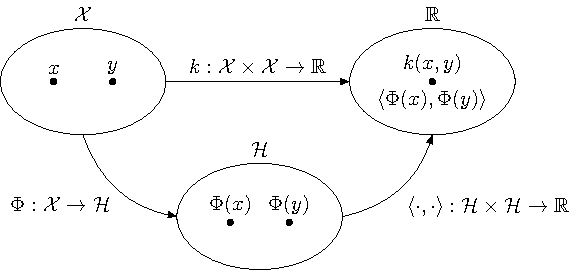
\includegraphics[]{figs/fig-kernel-map-diagram}
    \caption{Kernel map diagram.}
    \label{fig:kernel-map-diagram}
\end{figure}


Now, we want to restrict \(k\) so that it is a valid inner product.
Since inner products are symmetric and positive definite, it follows that \(k\) should have these properties as well.
Let \(S = \{x_1, x_2, \dots, x_n\} \subseteq X\) be a sample of points in \(X\).
We say \(K\) is the \textit{kernel matrix} of \(S\) with respect to \(k\) if \([K]_{ij} = k(x_i, x_j)\) for all \(i,j = 1,2,\dots, n\).
Then \(K\) should be equal to the Gram matrix of \(\Phi(S)\) with respect to \(\langle \cdot, \cdot \rangle\).
By \Cref{thm:gram-spsd}, \(K\) will be symmetric and positive semidefinite.

\begin{definition}[kernel]
    Let \(X\) be a nonempty set and \(k : X \times X \to \RR\).
    Then \(k\) is a (positive definite) \textit{kernel} if:
    \begin{enumerate}
        \item \(k\) is symmetric.
        For all \(x,y \in X\), \(k(x,y) = k(y,x)\).
        \item \(k\) is positive definite: if \(x_1, \dots, x_n \in X\) and \(c_1, \dots, c_n \in \RR\), then
        \[\sum_{i=1}^{n}\sum_{j=1}^{n} c_i c_j k(x_i, x_j) \geq 0.\]
        Equivalently, the kernel matrix \(K \in \RR^{n \times n}\) whose entries are \([K]_{ij} = k(x_i, x_j)\) is positive semidefinite, that is, \(\mathbf{c}^\top K \mathbf{c} \geq 0\) for all \(\mathbf{c} \in \RR^n\).
    \end{enumerate}
\end{definition}

% \subsubsection*{To do:}
% \begin{itemize}
%     \item move kernel/Gram matrix to its own definition
%     \item Define linear functionals
%     \item Define dual space (maybe?)
%     \item Riesz representation theorem
%     \item Define evaluation functionals
%     \item Define RKHS (continuous evaluation functionals)
%     \item An RKHS defines a unique reproducing kernel (by Riesz representation theorem).
%     \item Mercer's theorem.
%     \item A kernel defines a feature map.
%     \item A kernel defines a unique RKHS (by Mercer/Moore-Aronszajn).
%     \item We finally get \(k(x,y) = \langle \Phi(x), \Phi(y) \rangle_H\).
% \end{itemize}

\subsection{Constructing kernels}

\begin{theorem}
    \cite{rudin2020notes,shawe2004kernel}
    Suppose \(k_1\) and \(k_2\) are kernels over \(X \times X\).
    The following functions kernels.
    \begin{enumerate}
        \item \(k(x,y) = a_1 k_1(x,y) + a_2 k_2(x,y)\) for all \(a_1, a_2 \geq 0\).
        \item \(k(x,y) = k_1(x,y) k_2(x,y)\).
        \item \(k(x,y) = a_0 + a_1 k_1(x,y) + a_2 k_1(x,y)^2 + \cdots + a_n k_1(x,y)^n\) for all \(n \in \NN\) and \(a_0, \dots, a_n \geq 0\).
        \item \(k(x,y) = k_1(h(x),h(y))\) for all \(h : X \to X\).
        \item \(k(x,y) = g(x)g(y)\) for all \(g : X \to \RR\).
        \item \(k(x,y) = \exp(k_1(x,y))\).
    \end{enumerate}
\end{theorem}

\begin{proof}
    Let \(x_1, \dots, x_n \in X\) and \(c_1, \dots, c_n \in \RR\).
    \begin{enumerate}
        \item \label{itm:kernel-linear-combo}
        Let \(k = a_1k_1 + a_2k_2\) for \(a_1, a_2 \geq 0\).
        Since \(k_1\) and \(k_2\) are symmetric,
        \[
            k(x,y)
            = a_1k_1(x,y) + a_2k_2(x,y)
            = a_1k_1(y,x) + a_2k_2(y,x)
            = k(y,x),
        \]
        for all \(x,y \in X\).
        So, \(k\) is symmetric.

        Since \(k_1\) and \(k_2\) are positive semidefinite and \(a_1, a_2 \geq 0\),
        \begin{align*}
            \sum_{i=1}^{n} \sum_{j=1}^{n} c_i c_j k(x_i,x_j)
            &= \sum_{i=1}^{n} \sum_{j=1}^{n} c_i c_j (a_1 k_1(x_i,x_j) + a_2 k_2(x_i,x_j))\\
            &= a_1 \sum_{i=1}^{n} \sum_{j=1}^{n} c_i c_j k_1(x_i,x_j)
            + a_2 \sum_{i=1}^{n} \sum_{j=1}^{n} c_i c_j k_2(x_i,x_j)\\
            &\geq 0.
        \end{align*}
        So, \(k\) is positive semidefinite.
        \item \label{itm:kernel-product}
        Let \(k = k_1 k_2\).
        Define \(K\) so that \([K]_{ij} = k(x_i,x_j) = k_1(x_i, x_j) k_2(x_i, x_j)\).
        Let \(K_1\) and \(K_2\) be the Gram matrices for \(k_1\) and \(k_2\), respectively.
        Then \(K_1, K_2\) have orthonormal eigenvectors and nonnegative eigenvalues such that
        \def\dsum{\displaystyle\sum}
        \begin{align*}
            K_1 &= V LV^\top \\
            &= \begin{bmatrix}
                v_{11} & \cdots & v_{1n}\\
                \vdots & \ddots & \vdots\\
                v_{n1} & \cdots & v_{nn}\\
            \end{bmatrix}
            \begin{bmatrix}
                \lambda_{1} & \cdots & 0\\
                \vdots & \ddots & \vdots\\
                0 & \cdots & \lambda_{n}\\
            \end{bmatrix}
            \begin{bmatrix}
                v_{11} & \cdots & v_{n1}\\
                \vdots & \ddots & \vdots\\
                v_{1n} & \cdots & v_{nn}\\
            \end{bmatrix}\\
            &= \begin{bmatrix}
                \dsum_{j=1}^{n} \lambda_{j} v_{1j} v_{1j} & \cdots & \dsum_{j=1}^{n} \lambda_{j} v_{nj} v_{1j} \\
                \vdots & \ddots & \vdots\\
                \dsum_{j=1}^{n} \lambda_{j} v_{1j} v_{nj} & \cdots & \dsum_{j=1}^{n} \lambda_{j} v_{nj} v_{nj}\\
            \end{bmatrix}\\
            &= \sum_{j=1}^{n} \lambda_{j}
            \begin{bmatrix}
                v_{1j} v_{1j} & \cdots & v_{nj} v_{1j} \\
                \vdots & \ddots & \vdots\\
                v_{1j} v_{nj} & \cdots & v_{nj} v_{nj}\\
            \end{bmatrix}
            \intertext{and}
            K_2 &= UMU^\top = \sum_{j=1}^{n} \mu_{j}
            \begin{bmatrix}
                u_{1j} u_{1j} & \cdots & u_{nj} u_{1j} \\
                \vdots & \ddots & \vdots\\
                u_{1j} u_{nj} & \cdots & u_{nj} u_{nj}\\
            \end{bmatrix}.
        \end{align*}
        \def\v{\mathbf{v}}
        \def\u{\mathbf{u}}
        Let \(\v_i = \begin{bmatrix}
            v_{1i} & \cdots & v_{ni}
        \end{bmatrix}^\top\) and \(\u_j = \begin{bmatrix}
            u_{1j} & \cdots & u_{nj}
        \end{bmatrix}\), for all \(i,j = 1, 2, \dots, n\).
        Then
        \begin{align*}
            K &= K_1 \circ K_2\\
            &= \sum_{i=1}^{n} \lambda_{i}
            \begin{bmatrix}
                v_{1i} v_{1i} & \cdots & v_{ni} v_{1i} \\
                \vdots & \ddots & \vdots\\
                v_{1i} v_{ni} & \cdots & v_{ni} v_{ni}\\
            \end{bmatrix} \circ
            \sum_{j=1}^{n} \mu_{j}
            \begin{bmatrix}
                u_{1j} u_{1j} & \cdots & u_{nj} u_{1j} \\
                \vdots & \ddots & \vdots\\
                u_{1j} u_{nj} & \cdots & u_{nj} u_{nj}\\
            \end{bmatrix}\\
            &= \sum_{i=1}^{n} \sum_{j=1}^{n} \lambda_{i} \mu_{j}
            \begin{bmatrix}
                v_{1i} u_{1j} v_{1i} u_{1j} & \cdots & v_{1i} u_{1j} v_{ni} u_{nj} \\
                \vdots & \ddots & \vdots\\
                v_{ni} u_{nj} v_{1i} u_{1j} & \cdots & v_{ni} u_{nj} v_{ni}  u_{nj}
            \end{bmatrix}\\
            &= \sum_{i=1}^{n} \sum_{j=1}^{n} \lambda_{i} \mu_{j}
            \begin{bmatrix}
                v_{1i} u_{1j} \\ \vdots \\ v_{ni} u_{nj}
            \end{bmatrix}
            \begin{bmatrix}
                v_{1i} u_{1j} & \cdots & v_{ni} u_{nj}
            \end{bmatrix}\\
            &= \sum_{i=1}^{n} \sum_{j=1}^{n} \lambda_{i} \mu_{j}
            (\v_i \circ \u_j) (\v_i \circ \u_j)^\top,
        \end{align*}
        where \(\circ\) is the Hadamard product.
        Each \((\v_i \circ \u_j) (\v_i \circ \u_j)^\top\) is a symmetric positive semidefinite matrix.
        Since \(K_1, K_2\) are positive semidefinite, we have \(\lambda_i, \mu_i > 0\).
        Then \(K\) is symmetric positive semidefinite.
        \item By part \ref{itm:kernel-product}, \(k_1, k_1^2, \dots, k_1^n\) are kernels.
        By part \ref{itm:kernel-linear-combo}, \(a_0 + a_1 k_1 + a_2 k_1^2 + \dots + a_n k_1^n\) is a kernel.
        \item Since \(y_i = h(x_i) \in X\) for all \(i = 1,2,\dots, n\), we have
        \begin{align*}
            \sum_{i=1}^{n} \sum_{j=1}^{n} c_i c_j k(x_i,x_j)
            &= \sum_{i=1}^{n} \sum_{j=1}^{n} c_i c_j k_1(h(x_i), h(x_j))\\
            &= \sum_{i=1}^{n} \sum_{j=1}^{n} c_i c_j k_1(y_i, y_j)\\
            &\geq 0.
        \end{align*}
        \item Let \(g : X \to \RR\) and let \(c_i g(x_i) = y_i \in \RR\).
        If \(k(x,y) = g(x)g(y)\), then
        \begin{align*}
            \sum_{i=1}^{n} \sum_{j=1}^{n} c_i c_j k(x_i,x_j)
            &= \sum_{i=1}^{n} \sum_{j=1}^{n} c_i g(x_i) c_j g(x_j)\\
            &= \sum_{i=1}^{n} \sum_{j=1}^{n} y_i y_j\\
            % &= \sum_{\ell=1}^{n} \left(y_\ell^2 + \sum_{i=\ell+1}^{n} y_i y_\ell + \sum_{j=\ell+1}^{n} y_\ell y_j\right)\\
            % &= \sum_{i=1}^{n} \left(y_i^2 + 2\sum_{j=i+1}^{n} y_i y_j\right)\\
            &= \left(\sum_{i=1}^{n} y_i\right)^2\\
            &\geq 0.
        \end{align*}
        \item Let \(K_1\) be the Gram matrix for \(k_1\).
        If \(K_1 v = \lambda v\), then \(K_1^m = \lambda^m v\) for all \(m \in \NN\).
        So,
        \begin{align*}
            (\exp K_1) v
            = \sum_{m=0}^{\infty} \frac{K_1^m v}{m!}
            = \sum_{m=0}^{\infty} \frac{\lambda^m v}{m!}
            = e^\lambda v.
        \end{align*}
        Then \(K = \exp K_1\) has eigenvalues \(e^\lambda\).
        Since \(K_1\) is positive semidefinite, it has real eigenvalues so that \(e^\lambda > 0\).
        It follows that \(K\) is positive definite.
    \end{enumerate}
\end{proof}

\begin{theorem}[Gaussian kernel]
    \label{thm:gaussian-kernel}
    The function \(k : \RR^n \times \RR^n \to \RR\) defined by
    \[k(x,y) = \exp\left(\dfrac{-\|x-y\|^2_2}{\sigma^2}\right),\]
    is a kernel.
\end{theorem}

\begin{proof}
    
\end{proof}